% Axis D: median of the PER-INSTANCE ratio rev-A* / fwd-A* expansions.
% Computed from results/cluster/combined_long.csv over instances both solve.
% Per-instance-then-median, per the convention stated in the Metrics subsubsection.
% y positions are explicit numerics, bottom to top: descent 6, descent 26,
% sandstone 6, sandstone 26, plants 6, plants 26. Values must match the axis D prose.
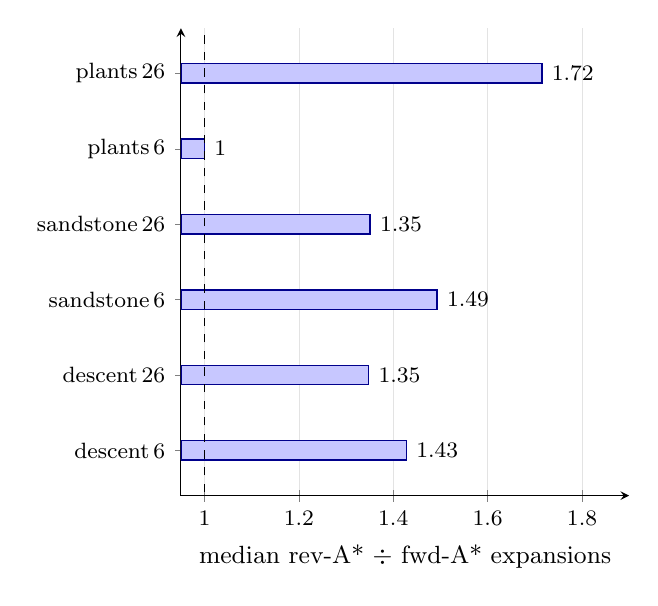
\begin{tikzpicture}
\begin{axis}[
  width=0.60\columnwidth, height=0.62\columnwidth,
  xbar,
  axis lines=left,
  xmin=0.95, xmax=1.90,
  xtick={1.0,1.2,1.4,1.6,1.8},
  xlabel={median rev-A* $\div$ fwd-A* expansions},
  label style={font=\small},
  tick label style={font=\footnotesize},
  ymin=0.4, ymax=6.6,
  ytick={1,2,3,4,5,6},
  yticklabels={descent\,6, descent\,26, sandstone\,6, sandstone\,26, plants\,6, plants\,26},
  y tick label style={font=\footnotesize},
  bar width=7pt,
  nodes near coords,
  nodes near coords style={font=\footnotesize, anchor=west,
                           /pgf/number format/fixed, /pgf/number format/precision=2},
  xmajorgrids, grid style={line width=.2pt, draw=gray!22},
]
\addplot[fill=blue!22, draw=blue!55!black, line width=.5pt]
  coordinates {(1.428,1) (1.348,2) (1.493,3) (1.351,4) (1.000,5) (1.715,6)};
% parity: the two directions expand the same set
\draw[black, dashed, line width=.6pt] (axis cs:1.0,0.45) -- (axis cs:1.0,6.55);
\end{axis}
\end{tikzpicture}
